\documentclass[openany]{book}
\usepackage{lmodern}
\usepackage{amssymb,amsmath}
\usepackage{ifxetex,ifluatex}
\usepackage{fixltx2e} % provides \textsubscript
\ifnum 0\ifxetex 1\fi\ifluatex 1\fi=0 % if pdftex
  \usepackage[T1]{fontenc}
  \usepackage[utf8]{inputenc}
\else % if luatex or xelatex
  \ifxetex
    \usepackage{mathspec}
  \else
    \usepackage{fontspec}
  \fi
  \defaultfontfeatures{Ligatures=TeX,Scale=MatchLowercase}
\fi
% use upquote if available, for straight quotes in verbatim environments
\IfFileExists{upquote.sty}{\usepackage{upquote}}{}
% use microtype if available
\IfFileExists{microtype.sty}{%
\usepackage{microtype}
\UseMicrotypeSet[protrusion]{basicmath} % disable protrusion for tt fonts
}{}
\usepackage[margin=1in]{geometry}
\usepackage{hyperref}
\hypersetup{unicode=true,
            pdftitle={Project One},
            pdfauthor={Vinicio Haro; Sang Yoon (Andy) Hwang; Julian McEachern; Jeremy O'Brien; Bethany Poulin},
            pdfborder={0 0 0},
            breaklinks=true}
\urlstyle{same}  % don't use monospace font for urls
\usepackage{natbib}
\bibliographystyle{apalike}
\usepackage{color}
\usepackage{fancyvrb}
\newcommand{\VerbBar}{|}
\newcommand{\VERB}{\Verb[commandchars=\\\{\}]}
\DefineVerbatimEnvironment{Highlighting}{Verbatim}{commandchars=\\\{\}}
% Add ',fontsize=\small' for more characters per line
\usepackage{framed}
\definecolor{shadecolor}{RGB}{248,248,248}
\newenvironment{Shaded}{\begin{snugshade}}{\end{snugshade}}
\newcommand{\AlertTok}[1]{\textcolor[rgb]{0.94,0.16,0.16}{#1}}
\newcommand{\AnnotationTok}[1]{\textcolor[rgb]{0.56,0.35,0.01}{\textbf{\textit{#1}}}}
\newcommand{\AttributeTok}[1]{\textcolor[rgb]{0.77,0.63,0.00}{#1}}
\newcommand{\BaseNTok}[1]{\textcolor[rgb]{0.00,0.00,0.81}{#1}}
\newcommand{\BuiltInTok}[1]{#1}
\newcommand{\CharTok}[1]{\textcolor[rgb]{0.31,0.60,0.02}{#1}}
\newcommand{\CommentTok}[1]{\textcolor[rgb]{0.56,0.35,0.01}{\textit{#1}}}
\newcommand{\CommentVarTok}[1]{\textcolor[rgb]{0.56,0.35,0.01}{\textbf{\textit{#1}}}}
\newcommand{\ConstantTok}[1]{\textcolor[rgb]{0.00,0.00,0.00}{#1}}
\newcommand{\ControlFlowTok}[1]{\textcolor[rgb]{0.13,0.29,0.53}{\textbf{#1}}}
\newcommand{\DataTypeTok}[1]{\textcolor[rgb]{0.13,0.29,0.53}{#1}}
\newcommand{\DecValTok}[1]{\textcolor[rgb]{0.00,0.00,0.81}{#1}}
\newcommand{\DocumentationTok}[1]{\textcolor[rgb]{0.56,0.35,0.01}{\textbf{\textit{#1}}}}
\newcommand{\ErrorTok}[1]{\textcolor[rgb]{0.64,0.00,0.00}{\textbf{#1}}}
\newcommand{\ExtensionTok}[1]{#1}
\newcommand{\FloatTok}[1]{\textcolor[rgb]{0.00,0.00,0.81}{#1}}
\newcommand{\FunctionTok}[1]{\textcolor[rgb]{0.00,0.00,0.00}{#1}}
\newcommand{\ImportTok}[1]{#1}
\newcommand{\InformationTok}[1]{\textcolor[rgb]{0.56,0.35,0.01}{\textbf{\textit{#1}}}}
\newcommand{\KeywordTok}[1]{\textcolor[rgb]{0.13,0.29,0.53}{\textbf{#1}}}
\newcommand{\NormalTok}[1]{#1}
\newcommand{\OperatorTok}[1]{\textcolor[rgb]{0.81,0.36,0.00}{\textbf{#1}}}
\newcommand{\OtherTok}[1]{\textcolor[rgb]{0.56,0.35,0.01}{#1}}
\newcommand{\PreprocessorTok}[1]{\textcolor[rgb]{0.56,0.35,0.01}{\textit{#1}}}
\newcommand{\RegionMarkerTok}[1]{#1}
\newcommand{\SpecialCharTok}[1]{\textcolor[rgb]{0.00,0.00,0.00}{#1}}
\newcommand{\SpecialStringTok}[1]{\textcolor[rgb]{0.31,0.60,0.02}{#1}}
\newcommand{\StringTok}[1]{\textcolor[rgb]{0.31,0.60,0.02}{#1}}
\newcommand{\VariableTok}[1]{\textcolor[rgb]{0.00,0.00,0.00}{#1}}
\newcommand{\VerbatimStringTok}[1]{\textcolor[rgb]{0.31,0.60,0.02}{#1}}
\newcommand{\WarningTok}[1]{\textcolor[rgb]{0.56,0.35,0.01}{\textbf{\textit{#1}}}}
\usepackage{longtable,booktabs}
\usepackage{graphicx,grffile}
\makeatletter
\def\maxwidth{\ifdim\Gin@nat@width>\linewidth\linewidth\else\Gin@nat@width\fi}
\def\maxheight{\ifdim\Gin@nat@height>\textheight\textheight\else\Gin@nat@height\fi}
\makeatother
% Scale images if necessary, so that they will not overflow the page
% margins by default, and it is still possible to overwrite the defaults
% using explicit options in \includegraphics[width, height, ...]{}
\setkeys{Gin}{width=\maxwidth,height=\maxheight,keepaspectratio}
\IfFileExists{parskip.sty}{%
\usepackage{parskip}
}{% else
\setlength{\parindent}{0pt}
\setlength{\parskip}{6pt plus 2pt minus 1pt}
}
\setlength{\emergencystretch}{3em}  % prevent overfull lines
\providecommand{\tightlist}{%
  \setlength{\itemsep}{0pt}\setlength{\parskip}{0pt}}
\setcounter{secnumdepth}{0}

%%% Use protect on footnotes to avoid problems with footnotes in titles
\let\rmarkdownfootnote\footnote%
\def\footnote{\protect\rmarkdownfootnote}

%%% Change title format to be more compact
\usepackage{titling}

% Create subtitle command for use in maketitle
\providecommand{\subtitle}[1]{
  \posttitle{
    \begin{center}\large#1\end{center}
    }
}

\setlength{\droptitle}{-2em}

  \title{Project One}
    \pretitle{\vspace{\droptitle}\centering\huge}
  \posttitle{\par}
  \subtitle{Group Two}
  \author{Vinicio Haro \\ Sang Yoon (Andy) Hwang \\ Julian McEachern \\ Jeremy O'Brien \\ Bethany Poulin}
    \preauthor{\centering\large\emph}
  \postauthor{\par}
      \predate{\centering\large\emph}
  \postdate{\par}
    \date{22 October 2019}

\usepackage{booktabs}
\usepackage[table]{xcolor}

% set plain style for page numbers
\pagestyle{plain}
\raggedbottom

% change font
\usepackage{fontspec}
\setmainfont{Arial}

% remove "chapter" from chapter title
\usepackage{titlesec}
\titleformat{\chapter}
  {\normalfont\LARGE\bfseries}{\thechapter}{1em}{}
\titlespacing*{\chapter}{0pt}{3.5ex plus 1ex minus .2ex}{2.3ex plus .2ex}

% create color block quotes
\usepackage{tcolorbox}
\newtcolorbox{myquote}{colback=orange!20!white, colframe=black!75!black}
\renewenvironment{quote}{\begin{myquote}}{\end{myquote}}

% wrap text
\usepackage{geometry}[textwidth=6in]

% kable 
\usepackage{tabu}
\usepackage{float}

\begin{document}
\maketitle

{
\setcounter{tocdepth}{1}
\tableofcontents
}
\hypertarget{overview}{%
\chapter*{Overview}\label{overview}}
\addcontentsline{toc}{chapter}{Overview}

Project 1 Overview. Explanation of process, etc.

\hypertarget{dependencies}{%
\section*{Dependencies}\label{dependencies}}
\addcontentsline{toc}{section}{Dependencies}

The following R libraries were used to complete Project 1.

\begin{Shaded}
\begin{Highlighting}[]
\CommentTok{# Processing}

\KeywordTok{library}\NormalTok{(readxl)}
\KeywordTok{library}\NormalTok{(tidyverse)}
\KeywordTok{library}\NormalTok{(zoo)}
\KeywordTok{library}\NormalTok{(janitor)}

\CommentTok{## Insert Additional Packages Here}

\CommentTok{# Graphing}
\KeywordTok{library}\NormalTok{(ggplot2)}
\KeywordTok{library}\NormalTok{(grid)}
\KeywordTok{library}\NormalTok{(gridExtra)}

\CommentTok{## Insert Additional Packages Here}

\CommentTok{# Timeseries }
\KeywordTok{library}\NormalTok{(zoo)}

\CommentTok{## Insert Additional Packages Here}

\CommentTok{# Math}
\KeywordTok{library}\NormalTok{(forecast)}
\KeywordTok{library}\NormalTok{(urca)}

\CommentTok{## Insert Additional Packages Here}

\CommentTok{# Formatting}
\KeywordTok{require}\NormalTok{(knitr)}
\KeywordTok{require}\NormalTok{(kableExtra)}
\KeywordTok{require}\NormalTok{(default)}
\end{Highlighting}
\end{Shaded}

\hypertarget{aquisition}{%
\section*{Data Aquisition}\label{aquisition}}
\addcontentsline{toc}{section}{Data Aquisition}

Data was stored within our group repository and imported below using the \texttt{readxl} package.

\begin{Shaded}
\begin{Highlighting}[]
\NormalTok{atm_data <-}\StringTok{ }\KeywordTok{read_excel}\NormalTok{(}\StringTok{"data/ATM624Data.xlsx"}\NormalTok{) }
\NormalTok{power_data <-}\StringTok{ }\KeywordTok{read_excel}\NormalTok{(}\StringTok{"data/ResidentialCustomerForecastLoad-624.xlsx"}\NormalTok{) }
\NormalTok{pipe1_data <-}\StringTok{ }\KeywordTok{read_excel}\NormalTok{(}\StringTok{"data/Waterflow_Pipe1.xlsx"}\NormalTok{)}
\NormalTok{pipe2_data <-}\StringTok{ }\KeywordTok{read_excel}\NormalTok{(}\StringTok{"data/Waterflow_Pipe2.xlsx"}\NormalTok{)}
\end{Highlighting}
\end{Shaded}

\hypertarget{part-a}{%
\chapter*{Part A: Forecasting ATM Withdrawals (JM)}\label{part-a}}
\addcontentsline{toc}{chapter}{Part A: Forecasting ATM Withdrawals (JM)}

\textbf{Juliann's Answer to \#1.}

\begin{quote}
\textbf{Instructions:} In part A, I want you to forecast how much cash is taken out of 4 different ATM machines for May 2010. The data is given in a single file. The variable \texttt{Cash} is provided in hundreds of dollars, other than that it is straight forward. I am being somewhat ambiguous on purpose. I am giving you data, please provide your written report on your findings, visuals, discussion and your R code all within a Word readable document, except the forecast which you will put in an Excel readable file. I must be able to cut and paste your R code and run it in R studio. Your report must be professional - most of all - readable, EASY to follow. Let me know what you are thinking, assumptions you are making! Your forecast is a simple CSV or Excel file that MATCHES the format of the data I provide.
\end{quote}

\hypertarget{a-exploration}{%
\section*{Exploration}\label{a-exploration}}
\addcontentsline{toc}{section}{Exploration}

Through data exploration, we identified that the original data file contained \texttt{NA} values in our \texttt{ATM} and \texttt{Cash} columns for 14 observations in May 2010. We removed these missing values and transformed the dataset into a wide format. Our cleaned dataframe was then converted into a timeseries format using the \texttt{zoo} package for forecasting in the next section. Our initial review of the data showed that ATM2 contained one missing value on 2009-10-25 and that ATM4 contained a potential outlier of \$1123 on 2010-02-09. We replaced both values with the corresponding mean value of each machine.

Next, we used a scatterplot to take an initial look at the correlation between cash withdrawals and dates for each machine. We can identified similiar patterns between ATM1 and ATM4, which show non-linear fluxuations that suggest a potential trend component in these timeseries. ATM2 follows a relatively linear path and decreases overtime. This changes in the last few observations, where withdrawals begin to increase. There are only 3 observed transactions for ATM3 that appear at the end of the captured time period.

\begin{Shaded}
\begin{Highlighting}[]
\CommentTok{# load data }
\NormalTok{atm_data <-}\StringTok{ }\KeywordTok{read_excel}\NormalTok{(}\StringTok{"data/ATM624Data.xlsx"}\NormalTok{) }

\CommentTok{# clean dataframe}
\NormalTok{atm <-}\StringTok{ }\NormalTok{atm_data }\OperatorTok\StringTok{ }
\StringTok{  }\CommentTok{# create wide dataframe}
\StringTok{  }\KeywordTok{spread}\NormalTok{(ATM, Cash) }\OperatorTok\StringTok{ }
\StringTok{  }\CommentTok{# remove NA column using function from janitor package}
\StringTok{  }\KeywordTok{remove_empty}\NormalTok{(}\DataTypeTok{which =} \StringTok{"cols"}\NormalTok{) }\OperatorTok
\StringTok{  }\CommentTok{# filter unobserved values from May 2010}
\StringTok{  }\KeywordTok{filter}\NormalTok{(DATE }\OperatorTok{<}\StringTok{ }\KeywordTok{as.Date}\NormalTok{(}\StringTok{"2010-05-01"}\NormalTok{)) }\OperatorTok
\StringTok{  }\CommentTok{# ensure dates are ascending}
\StringTok{  }\KeywordTok{arrange}\NormalTok{(DATE) }

\CommentTok{## remove NA}
\NormalTok{atm}\OperatorTok{$}\NormalTok{ATM2[}\KeywordTok{is.na}\NormalTok{(atm}\OperatorTok{$}\NormalTok{ATM2)] <-}\StringTok{ }\KeywordTok{mean}\NormalTok{(atm}\OperatorTok{$}\NormalTok{ATM2, }\DataTypeTok{na.rm =} \OtherTok{TRUE}\NormalTok{)}

\CommentTok{## remove outlier}
\NormalTok{atm}\OperatorTok{$}\NormalTok{ATM4[}\KeywordTok{which.max}\NormalTok{(atm}\OperatorTok{$}\NormalTok{ATM4)] <-}\StringTok{ }\KeywordTok{mean}\NormalTok{(atm}\OperatorTok{$}\NormalTok{ATM4, }\DataTypeTok{na.rm =} \OtherTok{TRUE}\NormalTok{)}

\CommentTok{# create time series   }
\NormalTok{atm_ts <-}\StringTok{ }\NormalTok{atm }\OperatorTok\StringTok{  }
\StringTok{  }\CommentTok{# remove column & generate date in timeseries using zoo}
\StringTok{  }\KeywordTok{select}\NormalTok{(}\OperatorTok{-}\NormalTok{DATE) }\OperatorTok\StringTok{ }
\StringTok{  }\CommentTok{# generate ts using zoo }
\StringTok{  }\KeywordTok{zoo}\NormalTok{(}\KeywordTok{seq}\NormalTok{(}\DataTypeTok{from =} \KeywordTok{as.Date}\NormalTok{(}\StringTok{"2009-05-01"}\NormalTok{), }\DataTypeTok{to =} \KeywordTok{as.Date}\NormalTok{(}\StringTok{"2010-05-14"}\NormalTok{), }\DataTypeTok{by =} \DecValTok{1}\NormalTok{))}

\CommentTok{# plot atms as scatterplot}
\NormalTok{atm }\OperatorTok\StringTok{ }
\StringTok{  }\CommentTok{# re-gather observations for facet plot}
\StringTok{  }\KeywordTok{gather}\NormalTok{(}\DataTypeTok{key=}\NormalTok{ATM, }\DataTypeTok{value=}\NormalTok{Cash, ATM1,ATM2, ATM3,ATM4) }\OperatorTok\StringTok{ }
\StringTok{  }\CommentTok{# remove NA value from ATM2}
\StringTok{  }\KeywordTok{filter}\NormalTok{(}\KeywordTok{complete.cases}\NormalTok{(.)) }\OperatorTok\StringTok{ }
\StringTok{  }\CommentTok{# plot }
\StringTok{  }\KeywordTok{ggplot}\NormalTok{(}\KeywordTok{aes}\NormalTok{(DATE, Cash, }\DataTypeTok{color=}\NormalTok{ATM)) }\OperatorTok{+}
\StringTok{  }\KeywordTok{geom_point}\NormalTok{() }\OperatorTok{+}
\StringTok{  }\KeywordTok{geom_smooth}\NormalTok{(}\DataTypeTok{method=}\StringTok{"loess"}\NormalTok{) }\OperatorTok{+}
\StringTok{  }\KeywordTok{facet_wrap}\NormalTok{(}\OperatorTok{~}\NormalTok{ATM, }\DataTypeTok{scales=}\StringTok{'free_x'}\NormalTok{, }\DataTypeTok{nrow=}\DecValTok{1}\NormalTok{) }\OperatorTok{+}
\StringTok{  }\KeywordTok{labs}\NormalTok{(}\DataTypeTok{title=}\StringTok{"ATM Scatterplot"}\NormalTok{)}\OperatorTok{+}
\StringTok{  }\KeywordTok{theme_bw}\NormalTok{()}\OperatorTok{+}
\StringTok{  }\KeywordTok{theme}\NormalTok{(}\DataTypeTok{legend.position =} \StringTok{'none'}\NormalTok{)}\OperatorTok{+}
\StringTok{  }\KeywordTok{scale_color_brewer}\NormalTok{()}
\end{Highlighting}
\end{Shaded}

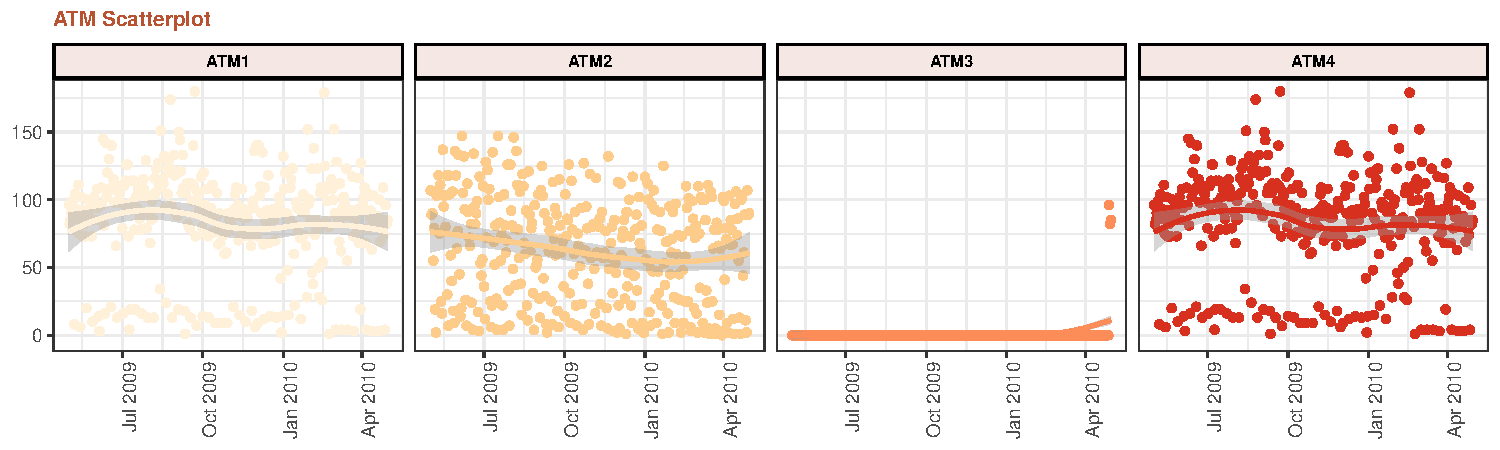
\includegraphics{project-one_files/figure-latex/unnamed-chunk-3-1.pdf}

\hypertarget{forecast}{%
\section{Forecast}\label{forecast}}

We subsetted each atm series to apply unique forecasting methods based on the observed data.

\hypertarget{atm1}{%
\subsection{ATM1}\label{atm1}}

\begin{Shaded}
\begin{Highlighting}[]
\CommentTok{#subset data }
\NormalTok{ATM1 <-}\StringTok{ }\NormalTok{atm_ts[,}\DecValTok{1}\NormalTok{]}

\CommentTok{#differentiated}
\NormalTok{ATM1d <-}\StringTok{  }\KeywordTok{diff}\NormalTok{(ATM1)}

\NormalTok{p1<-}\KeywordTok{autoplot}\NormalTok{(ATM1)}\OperatorTok{+}\StringTok{ }\KeywordTok{labs}\NormalTok{(}\DataTypeTok{title=}\StringTok{"Series: ATM1"}\NormalTok{)}\OperatorTok{+}\StringTok{ }
\StringTok{  }\KeywordTok{theme_bw}\NormalTok{()}\OperatorTok{+}\KeywordTok{theme}\NormalTok{()}
\NormalTok{p2<-}\KeywordTok{ggAcf}\NormalTok{(ATM1)}\OperatorTok{+}\StringTok{ }\KeywordTok{labs}\NormalTok{(}\DataTypeTok{title=}\StringTok{"Acf: ATM1"}\NormalTok{)}\OperatorTok{+}\StringTok{ }
\StringTok{  }\KeywordTok{theme_bw}\NormalTok{()}\OperatorTok{+}\KeywordTok{theme}\NormalTok{()}
\NormalTok{p3<-}\KeywordTok{ggPacf}\NormalTok{(ATM1)}\OperatorTok{+}\StringTok{ }\KeywordTok{labs}\NormalTok{(}\DataTypeTok{title=}\StringTok{"Pacf: ATM1"}\NormalTok{)}\OperatorTok{+}\StringTok{ }
\StringTok{  }\KeywordTok{theme_bw}\NormalTok{()}\OperatorTok{+}\KeywordTok{theme}\NormalTok{()}
\NormalTok{p4<-}\KeywordTok{autoplot}\NormalTok{(ATM1d)}\OperatorTok{+}\StringTok{ }\KeywordTok{labs}\NormalTok{(}\DataTypeTok{title=}\StringTok{"Series: diff(ATM1)"}\NormalTok{)}\OperatorTok{+}\StringTok{ }
\StringTok{  }\KeywordTok{theme_bw}\NormalTok{()}\OperatorTok{+}\KeywordTok{theme}\NormalTok{()}
\NormalTok{p5<-}\KeywordTok{ggAcf}\NormalTok{(ATM1d)}\OperatorTok{+}\StringTok{ }\KeywordTok{labs}\NormalTok{(}\DataTypeTok{title=}\StringTok{"Acf: diff(ATM1)"}\NormalTok{)}\OperatorTok{+}\StringTok{ }
\StringTok{  }\KeywordTok{theme_bw}\NormalTok{()}\OperatorTok{+}\KeywordTok{theme}\NormalTok{()}
\NormalTok{p6<-}\KeywordTok{ggPacf}\NormalTok{(ATM1d)}\OperatorTok{+}\StringTok{ }\KeywordTok{labs}\NormalTok{(}\DataTypeTok{title=}\StringTok{"Pacf: diff(ATM1)"}\NormalTok{)}\OperatorTok{+}\StringTok{ }
\StringTok{  }\KeywordTok{theme_bw}\NormalTok{()}\OperatorTok{+}\KeywordTok{theme}\NormalTok{()}

\KeywordTok{grid.arrange}\NormalTok{(}\DataTypeTok{grob=}\NormalTok{p1, p4, p2, p5, p3, p6,}
             \DataTypeTok{ncol=}\DecValTok{2}\NormalTok{,}
             \DataTypeTok{top=}\KeywordTok{textGrob}\NormalTok{(}\StringTok{"Daily ATM Transactions for ATM1"}\NormalTok{,}
                          \DataTypeTok{gp =} \KeywordTok{gpar}\NormalTok{(}\DataTypeTok{fontface =} \StringTok{"bold"}\NormalTok{, }\DataTypeTok{cex =} \DecValTok{1}\NormalTok{)))}
\end{Highlighting}
\end{Shaded}

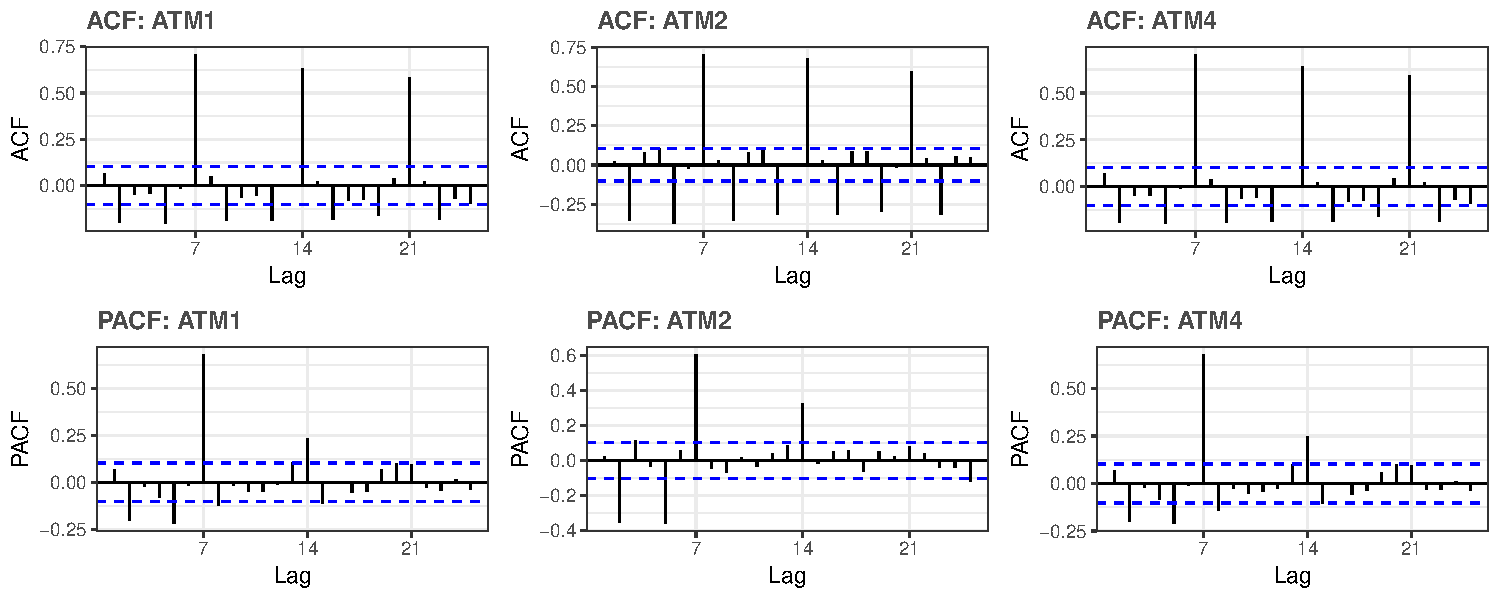
\includegraphics{project-one_files/figure-latex/unnamed-chunk-4-1.pdf}

\begin{Shaded}
\begin{Highlighting}[]
\CommentTok{# root test using urca package}
\NormalTok{ATM1 }\OperatorTok\StringTok{ }\KeywordTok{diff}\NormalTok{() }\OperatorTok\StringTok{ }\KeywordTok{ur.kpss}\NormalTok{() }\OperatorTok\StringTok{ }\KeywordTok{summary}\NormalTok{()}
\end{Highlighting}
\end{Shaded}

\begin{verbatim}
FALSE 
FALSE ####################### 
FALSE # KPSS Unit Root Test # 
FALSE ####################### 
FALSE 
FALSE Test is of type: mu with 5 lags. 
FALSE 
FALSE Value of test-statistic is: 0.0168 
FALSE 
FALSE Critical value for a significance level of: 
FALSE                 10pct  5pct 2.5pct  1pct
FALSE critical values 0.347 0.463  0.574 0.739
\end{verbatim}

\begin{Shaded}
\begin{Highlighting}[]
\NormalTok{ATM1d }\OperatorTok\StringTok{ }\KeywordTok{diff}\NormalTok{() }\OperatorTok\StringTok{ }\KeywordTok{ur.kpss}\NormalTok{() }\OperatorTok\StringTok{ }\KeywordTok{summary}\NormalTok{()}
\end{Highlighting}
\end{Shaded}

\begin{verbatim}
FALSE 
FALSE ####################### 
FALSE # KPSS Unit Root Test # 
FALSE ####################### 
FALSE 
FALSE Test is of type: mu with 5 lags. 
FALSE 
FALSE Value of test-statistic is: 0.011 
FALSE 
FALSE Critical value for a significance level of: 
FALSE                 10pct  5pct 2.5pct  1pct
FALSE critical values 0.347 0.463  0.574 0.739
\end{verbatim}

Our Acf plot for the ATM1 timeseries shows three large, decreasing lags at 7, 14, and 21. This confirms our assumption about seasonality within our observed data. Our data is non-stationary and should be differentiated in order to forecast the data using a seasonal ARIMA model.

\hypertarget{atm2}{%
\subsection{ATM2}\label{atm2}}

\begin{Shaded}
\begin{Highlighting}[]
\CommentTok{#subset data }
\NormalTok{ATM2 <-}\StringTok{ }\NormalTok{atm_ts[,}\DecValTok{2}\NormalTok{]}

\NormalTok{p1<-}\KeywordTok{autoplot}\NormalTok{(ATM2)}\OperatorTok{+}\StringTok{ }\KeywordTok{labs}\NormalTok{(}\DataTypeTok{title=}\StringTok{"Series: ATM2"}\NormalTok{)}\OperatorTok{+}\StringTok{ }\KeywordTok{theme_bw}\NormalTok{()}\OperatorTok{+}\KeywordTok{theme}\NormalTok{()}
\NormalTok{p2<-}\KeywordTok{ggAcf}\NormalTok{(ATM2)}\OperatorTok{+}\StringTok{ }\KeywordTok{labs}\NormalTok{(}\DataTypeTok{title=}\StringTok{"Acf: ATM2"}\NormalTok{)}\OperatorTok{+}\StringTok{ }\KeywordTok{theme_bw}\NormalTok{()}\OperatorTok{+}\KeywordTok{theme}\NormalTok{()}
\NormalTok{p3<-}\KeywordTok{ggPacf}\NormalTok{(ATM2)}\OperatorTok{+}\StringTok{ }\KeywordTok{labs}\NormalTok{(}\DataTypeTok{title=}\StringTok{"Pacf: ATM2"}\NormalTok{)}\OperatorTok{+}\StringTok{ }\KeywordTok{theme_bw}\NormalTok{()}\OperatorTok{+}\KeywordTok{theme}\NormalTok{()}

\KeywordTok{grid.arrange}\NormalTok{(}\DataTypeTok{grob=}\NormalTok{p1, p2, p3,}
             \DataTypeTok{layout_matrix =} \KeywordTok{rbind}\NormalTok{(}\KeywordTok{c}\NormalTok{(}\DecValTok{1}\NormalTok{,}\DecValTok{1}\NormalTok{),}\KeywordTok{c}\NormalTok{(}\DecValTok{2}\NormalTok{,}\DecValTok{3}\NormalTok{)),}
             \DataTypeTok{top=}\KeywordTok{textGrob}\NormalTok{(}\StringTok{"Daily ATM Transactions for ATM2"}\NormalTok{,}
                          \DataTypeTok{gp =} \KeywordTok{gpar}\NormalTok{(}\DataTypeTok{fontface =} \StringTok{"bold"}\NormalTok{, }\DataTypeTok{cex =} \DecValTok{1}\NormalTok{, }\DataTypeTok{col =} \StringTok{"#233c49"}\NormalTok{)))}
\end{Highlighting}
\end{Shaded}

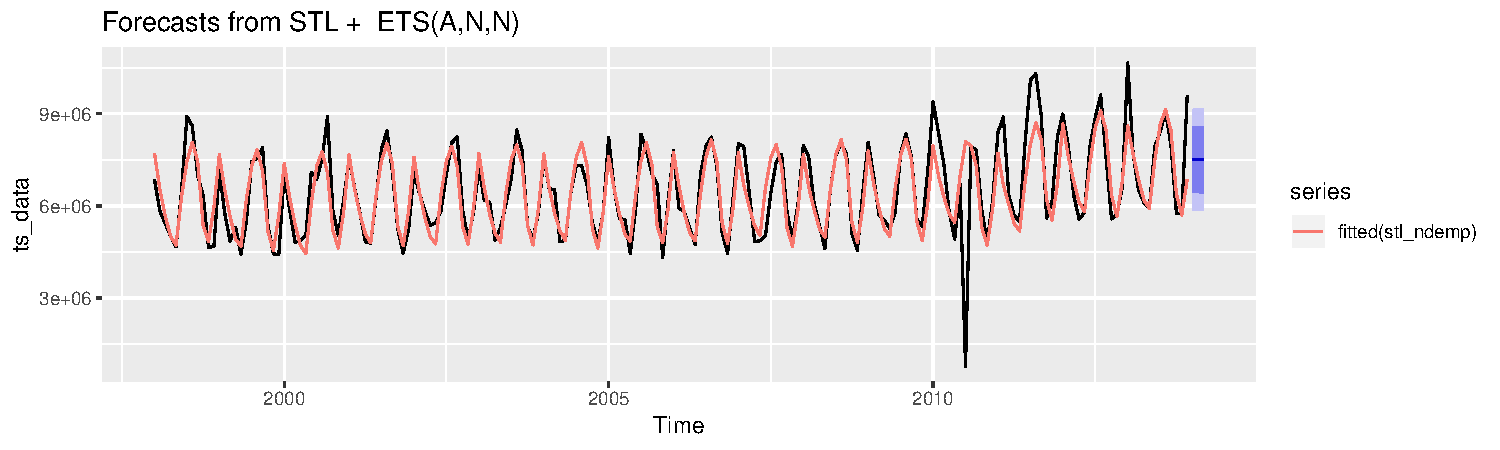
\includegraphics{project-one_files/figure-latex/unnamed-chunk-5-1.pdf}

\hypertarget{atm3}{%
\subsection{ATM3}\label{atm3}}

\begin{Shaded}
\begin{Highlighting}[]
\CommentTok{#subset data }
\NormalTok{ATM3 <-}\StringTok{ }\NormalTok{atm_ts[,}\DecValTok{3}\NormalTok{]}

\NormalTok{p1<-}\KeywordTok{autoplot}\NormalTok{(ATM3)}\OperatorTok{+}\StringTok{ }\KeywordTok{labs}\NormalTok{(}\DataTypeTok{title=}\StringTok{"Series: ATM3"}\NormalTok{)}\OperatorTok{+}\StringTok{ }\KeywordTok{theme_bw}\NormalTok{()}\OperatorTok{+}\KeywordTok{theme}\NormalTok{()}
\NormalTok{p2<-}\KeywordTok{ggAcf}\NormalTok{(ATM3)}\OperatorTok{+}\StringTok{ }\KeywordTok{labs}\NormalTok{(}\DataTypeTok{title=}\StringTok{"Acf: ATM3"}\NormalTok{)}\OperatorTok{+}\StringTok{ }\KeywordTok{theme_bw}\NormalTok{()}\OperatorTok{+}\KeywordTok{theme}\NormalTok{()}
\NormalTok{p3<-}\KeywordTok{ggPacf}\NormalTok{(ATM3)}\OperatorTok{+}\StringTok{ }\KeywordTok{labs}\NormalTok{(}\DataTypeTok{title=}\StringTok{"Pacf: ATM3"}\NormalTok{)}\OperatorTok{+}\StringTok{ }\KeywordTok{theme_bw}\NormalTok{()}\OperatorTok{+}\KeywordTok{theme}\NormalTok{()}

\KeywordTok{grid.arrange}\NormalTok{(}\DataTypeTok{grob=}\NormalTok{p1, p2, p3,}
             \DataTypeTok{layout_matrix =} \KeywordTok{rbind}\NormalTok{(}\KeywordTok{c}\NormalTok{(}\DecValTok{1}\NormalTok{,}\DecValTok{1}\NormalTok{),}\KeywordTok{c}\NormalTok{(}\DecValTok{2}\NormalTok{,}\DecValTok{3}\NormalTok{)),}
             \DataTypeTok{top=}\KeywordTok{textGrob}\NormalTok{(}\StringTok{"Daily ATM Transactions for ATM3"}\NormalTok{,}
                          \DataTypeTok{gp =} \KeywordTok{gpar}\NormalTok{(}\DataTypeTok{fontface =} \StringTok{"bold"}\NormalTok{, }\DataTypeTok{cex =} \DecValTok{1}\NormalTok{, }\DataTypeTok{col =} \StringTok{"#233c49"}\NormalTok{)))}
\end{Highlighting}
\end{Shaded}

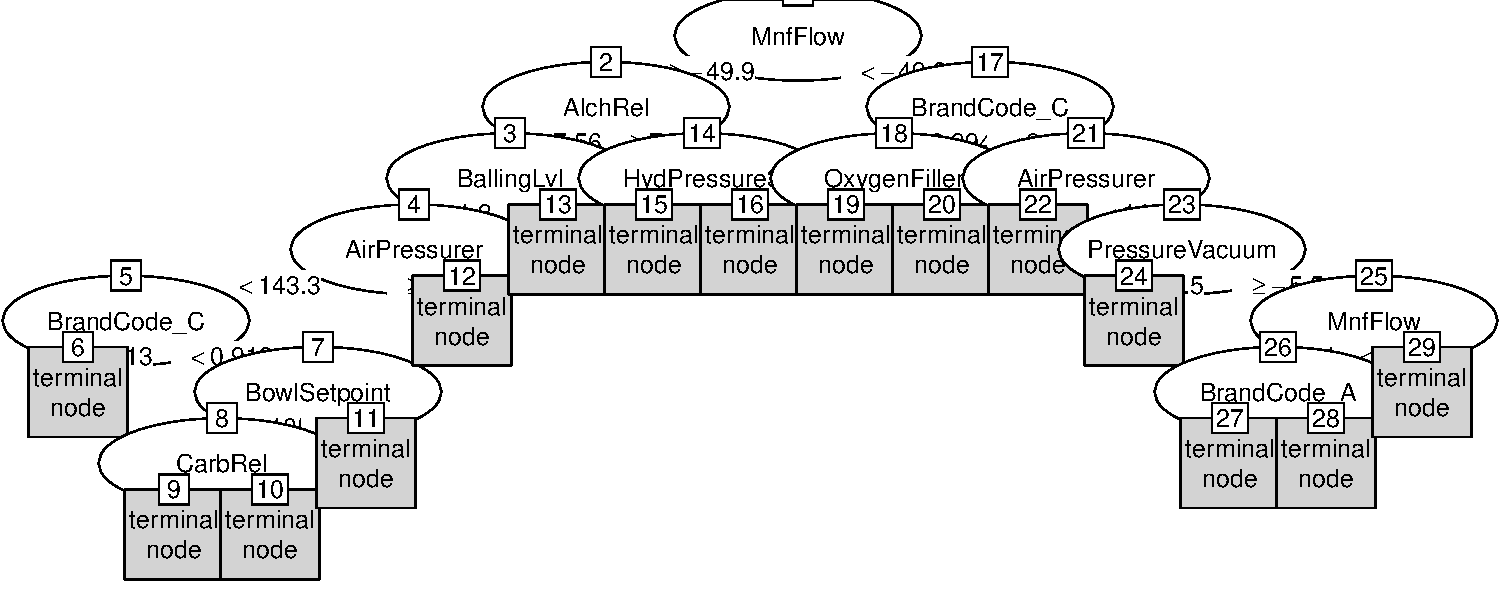
\includegraphics{project-one_files/figure-latex/unnamed-chunk-6-1.pdf}

\hypertarget{atm4}{%
\subsection{ATM4}\label{atm4}}

\begin{Shaded}
\begin{Highlighting}[]
\CommentTok{#subset data }
\NormalTok{ATM4 <-}\StringTok{ }\NormalTok{atm_ts[,}\DecValTok{4}\NormalTok{]}

\NormalTok{p1<-}\KeywordTok{autoplot}\NormalTok{(ATM4)}\OperatorTok{+}\StringTok{ }\KeywordTok{labs}\NormalTok{(}\DataTypeTok{title=}\StringTok{"Series: ATM4"}\NormalTok{)}\OperatorTok{+}\StringTok{ }\KeywordTok{theme_bw}\NormalTok{()}\OperatorTok{+}\KeywordTok{theme}\NormalTok{()}
\NormalTok{p2<-}\KeywordTok{ggAcf}\NormalTok{(ATM4)}\OperatorTok{+}\StringTok{ }\KeywordTok{labs}\NormalTok{(}\DataTypeTok{title=}\StringTok{"Acf: ATM4"}\NormalTok{)}\OperatorTok{+}\StringTok{ }\KeywordTok{theme_bw}\NormalTok{()}\OperatorTok{+}\KeywordTok{theme}\NormalTok{()}
\NormalTok{p3<-}\KeywordTok{ggPacf}\NormalTok{(ATM4)}\OperatorTok{+}\StringTok{ }\KeywordTok{labs}\NormalTok{(}\DataTypeTok{title=}\StringTok{"Pacf: ATM4"}\NormalTok{)}\OperatorTok{+}\StringTok{ }\KeywordTok{theme_bw}\NormalTok{()}\OperatorTok{+}\KeywordTok{theme}\NormalTok{()}

\KeywordTok{grid.arrange}\NormalTok{(}\DataTypeTok{grob=}\NormalTok{p1, p2, p3,}
             \DataTypeTok{layout_matrix =} \KeywordTok{rbind}\NormalTok{(}\KeywordTok{c}\NormalTok{(}\DecValTok{1}\NormalTok{,}\DecValTok{1}\NormalTok{),}\KeywordTok{c}\NormalTok{(}\DecValTok{2}\NormalTok{,}\DecValTok{3}\NormalTok{)),}
             \DataTypeTok{top=}\KeywordTok{textGrob}\NormalTok{(}\StringTok{"Daily ATM Transactions for ATM4"}\NormalTok{,}
                          \DataTypeTok{gp =} \KeywordTok{gpar}\NormalTok{(}\DataTypeTok{fontface =} \StringTok{"bold"}\NormalTok{, }\DataTypeTok{cex =} \DecValTok{1}\NormalTok{, }\DataTypeTok{col =} \StringTok{"#233c49"}\NormalTok{)))}
\end{Highlighting}
\end{Shaded}

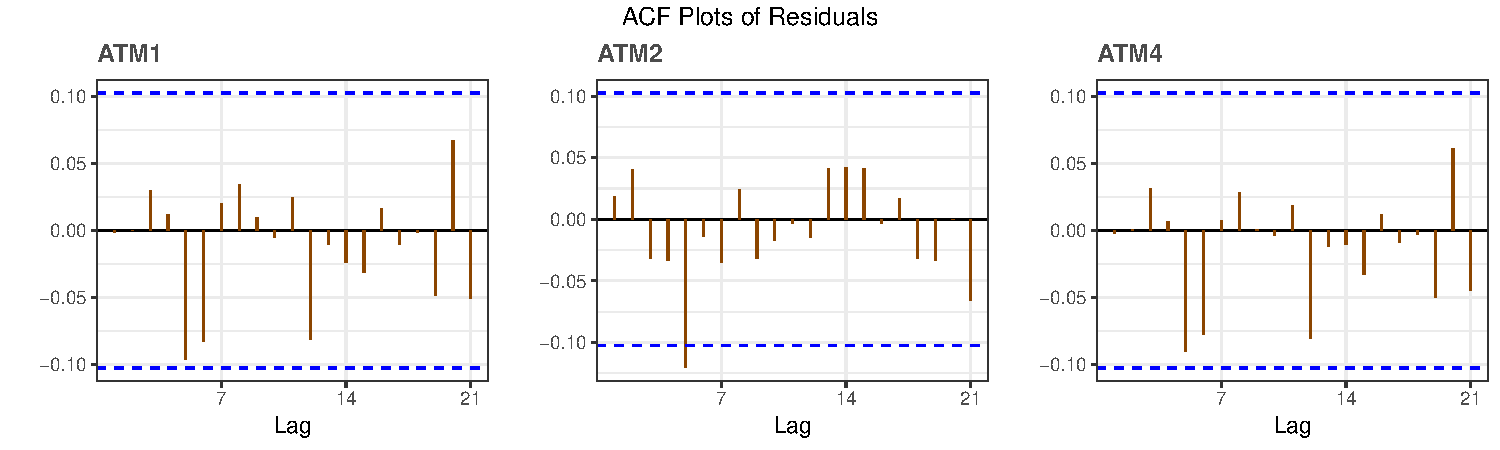
\includegraphics{project-one_files/figure-latex/unnamed-chunk-7-1.pdf}

\hypertarget{a-forecast}{%
\section*{Forecast}\label{a-forecast}}
\addcontentsline{toc}{section}{Forecast}

Data forecast.

\hypertarget{a-discussion}{%
\section*{Discussion}\label{a-discussion}}
\addcontentsline{toc}{section}{Discussion}

Discuss findings.

\hypertarget{part-a}{%
\chapter*{Part A: Forecasting ATM Withdrawals}\label{part-a}}
\addcontentsline{toc}{chapter}{Part A: Forecasting ATM Withdrawals}

\begin{quote}
\textbf{Instructions:} In part A, I want you to forecast how much cash is taken out of 4 different ATM machines for May 2010. The data is given in a single file. The variable \texttt{Cash} is provided in hundreds of dollars, other than that it is straight forward. I am being somewhat ambiguous on purpose. I am giving you data, please provide your written report on your findings, visuals, discussion and your R code all within a Word readable document, except the forecast which you will put in an Excel readable file. I must be able to cut and paste your R code and run it in R studio. Your report must be professional - most of all - readable, EASY to follow. Let me know what you are thinking, assumptions you are making! Your forecast is a simple CSV or Excel file that MATCHES the format of the data I provide.
\end{quote}

\hypertarget{a-exploration}{%
\section*{Exploration}\label{a-exploration}}
\addcontentsline{toc}{section}{Exploration}

\begin{Shaded}
\begin{Highlighting}[]
\NormalTok{atm_data <-}\StringTok{ }\KeywordTok{read_excel}\NormalTok{(}\StringTok{"data/ATM624Data.xlsx"}\NormalTok{) }
\end{Highlighting}
\end{Shaded}

Data exploration.

\hypertarget{a-forecast}{%
\section*{Forecast}\label{a-forecast}}
\addcontentsline{toc}{section}{Forecast}

Data forecast.

\hypertarget{a-discussion}{%
\section*{Discussion}\label{a-discussion}}
\addcontentsline{toc}{section}{Discussion}

Discuss findings.

\hypertarget{part-b}{%
\chapter*{Part B: Forecasting Power}\label{part-b}}
\addcontentsline{toc}{chapter}{Part B: Forecasting Power}

\begin{quote}
\textbf{Instructions:} Part B consists of a simple dataset of residential power usage for January 1998 until December 2013. Your assignment is to model these data and a monthly forecast for 2014. The data is given in a single file. The variable `KWH' is power consumption in Kilowatt hours, the rest is straight forward. Add these to your existing files above - clearly labeled.
\end{quote}

\hypertarget{b-exploration}{%
\section*{Data Exploration}\label{b-exploration}}
\addcontentsline{toc}{section}{Data Exploration}

Explore data.

\begin{Shaded}
\begin{Highlighting}[]
\NormalTok{power_data <-}\StringTok{ }\KeywordTok{read_excel}\NormalTok{(}\StringTok{"data/ResidentialCustomerForecastLoad-624.xlsx"}\NormalTok{) }
\end{Highlighting}
\end{Shaded}

\hypertarget{b-model}{%
\section*{Data Model}\label{b-model}}
\addcontentsline{toc}{section}{Data Model}

Model data.

\hypertarget{b-forecast}{%
\section*{Forecast}\label{b-forecast}}
\addcontentsline{toc}{section}{Forecast}

Data forecast.

\hypertarget{b-discussion}{%
\section*{Discussion}\label{b-discussion}}
\addcontentsline{toc}{section}{Discussion}

Discuss findings.

\hypertarget{part-C}{%
\chapter*{Part C: Forecasting Waterflow}\label{part-C}}
\addcontentsline{toc}{chapter}{Part C: Forecasting Waterflow}

\begin{quote}
\textbf{Instructions:} Part C consists of two data sets. These are simple 2 columns sets, however they have different time stamps. Your optional assignment is to time-base sequence the data and aggregate based on hour (example of what this looks like, follows). Note for multiple recordings within an hour, take the mean. Then to test appropriate assumptions and forecast a week forward with confidence bands (80 and 95\%). Add these to your existing files above - clearly labeled.
\end{quote}

\hypertarget{c-exploration}{%
\section*{Data Exploration}\label{c-exploration}}
\addcontentsline{toc}{section}{Data Exploration}

\begin{Shaded}
\begin{Highlighting}[]
\NormalTok{pipe1_data <-}\StringTok{ }\KeywordTok{read_excel}\NormalTok{(}\StringTok{"data/Waterflow_Pipe1.xlsx"}\NormalTok{)}
\NormalTok{pipe2_data <-}\StringTok{ }\KeywordTok{read_excel}\NormalTok{(}\StringTok{"data/Waterflow_Pipe2.xlsx"}\NormalTok{)}
\end{Highlighting}
\end{Shaded}

\hypertarget{c-model}{%
\section*{Time-Based Sequence}\label{c-model}}
\addcontentsline{toc}{section}{Time-Based Sequence}

Create time-based sequence.

\hypertarget{c-forecast}{%
\section*{Forecast}\label{c-forecast}}
\addcontentsline{toc}{section}{Forecast}

Data forecast.

\hypertarget{c-discussion}{%
\section*{Discussion}\label{c-discussion}}
\addcontentsline{toc}{section}{Discussion}

Discuss findings.

\bibliography{book.bib,packages.bib}


\end{document}
